% Frames!

% Bite => FUN? Evt et mere relevant attack fra virkeligheden (Laes EMV standarden og maaske tage den med som movitvation for at implementere disse countermeasures)
\begin{frame}{Why is it Important?}
\begin{itemize}
\item Smart cards is widespread in e.g. the banking industry
\item Countermeasures may be used for other embedded systems
  \begin{itemize}
  \item Air planes
  \item Satellites 
  \end{itemize}
\item Research in one area may help in other areas as well
\end{itemize}  
\end{frame}


% Java Card => Arkitektur (den firkantede figur), BCV, Firewall, JCVM eksekverer bytecode direkte og laver ikke JIT compilering

\section{Java Card}
\label{sec:java-card}
\begin{frame}{Java Card}
  \begin{itemize}
  \item Variation of a smart card
  \item Small in size
  \item Often used for access or paying
  \end{itemize}
\begin{figure}[h]
  \centering
  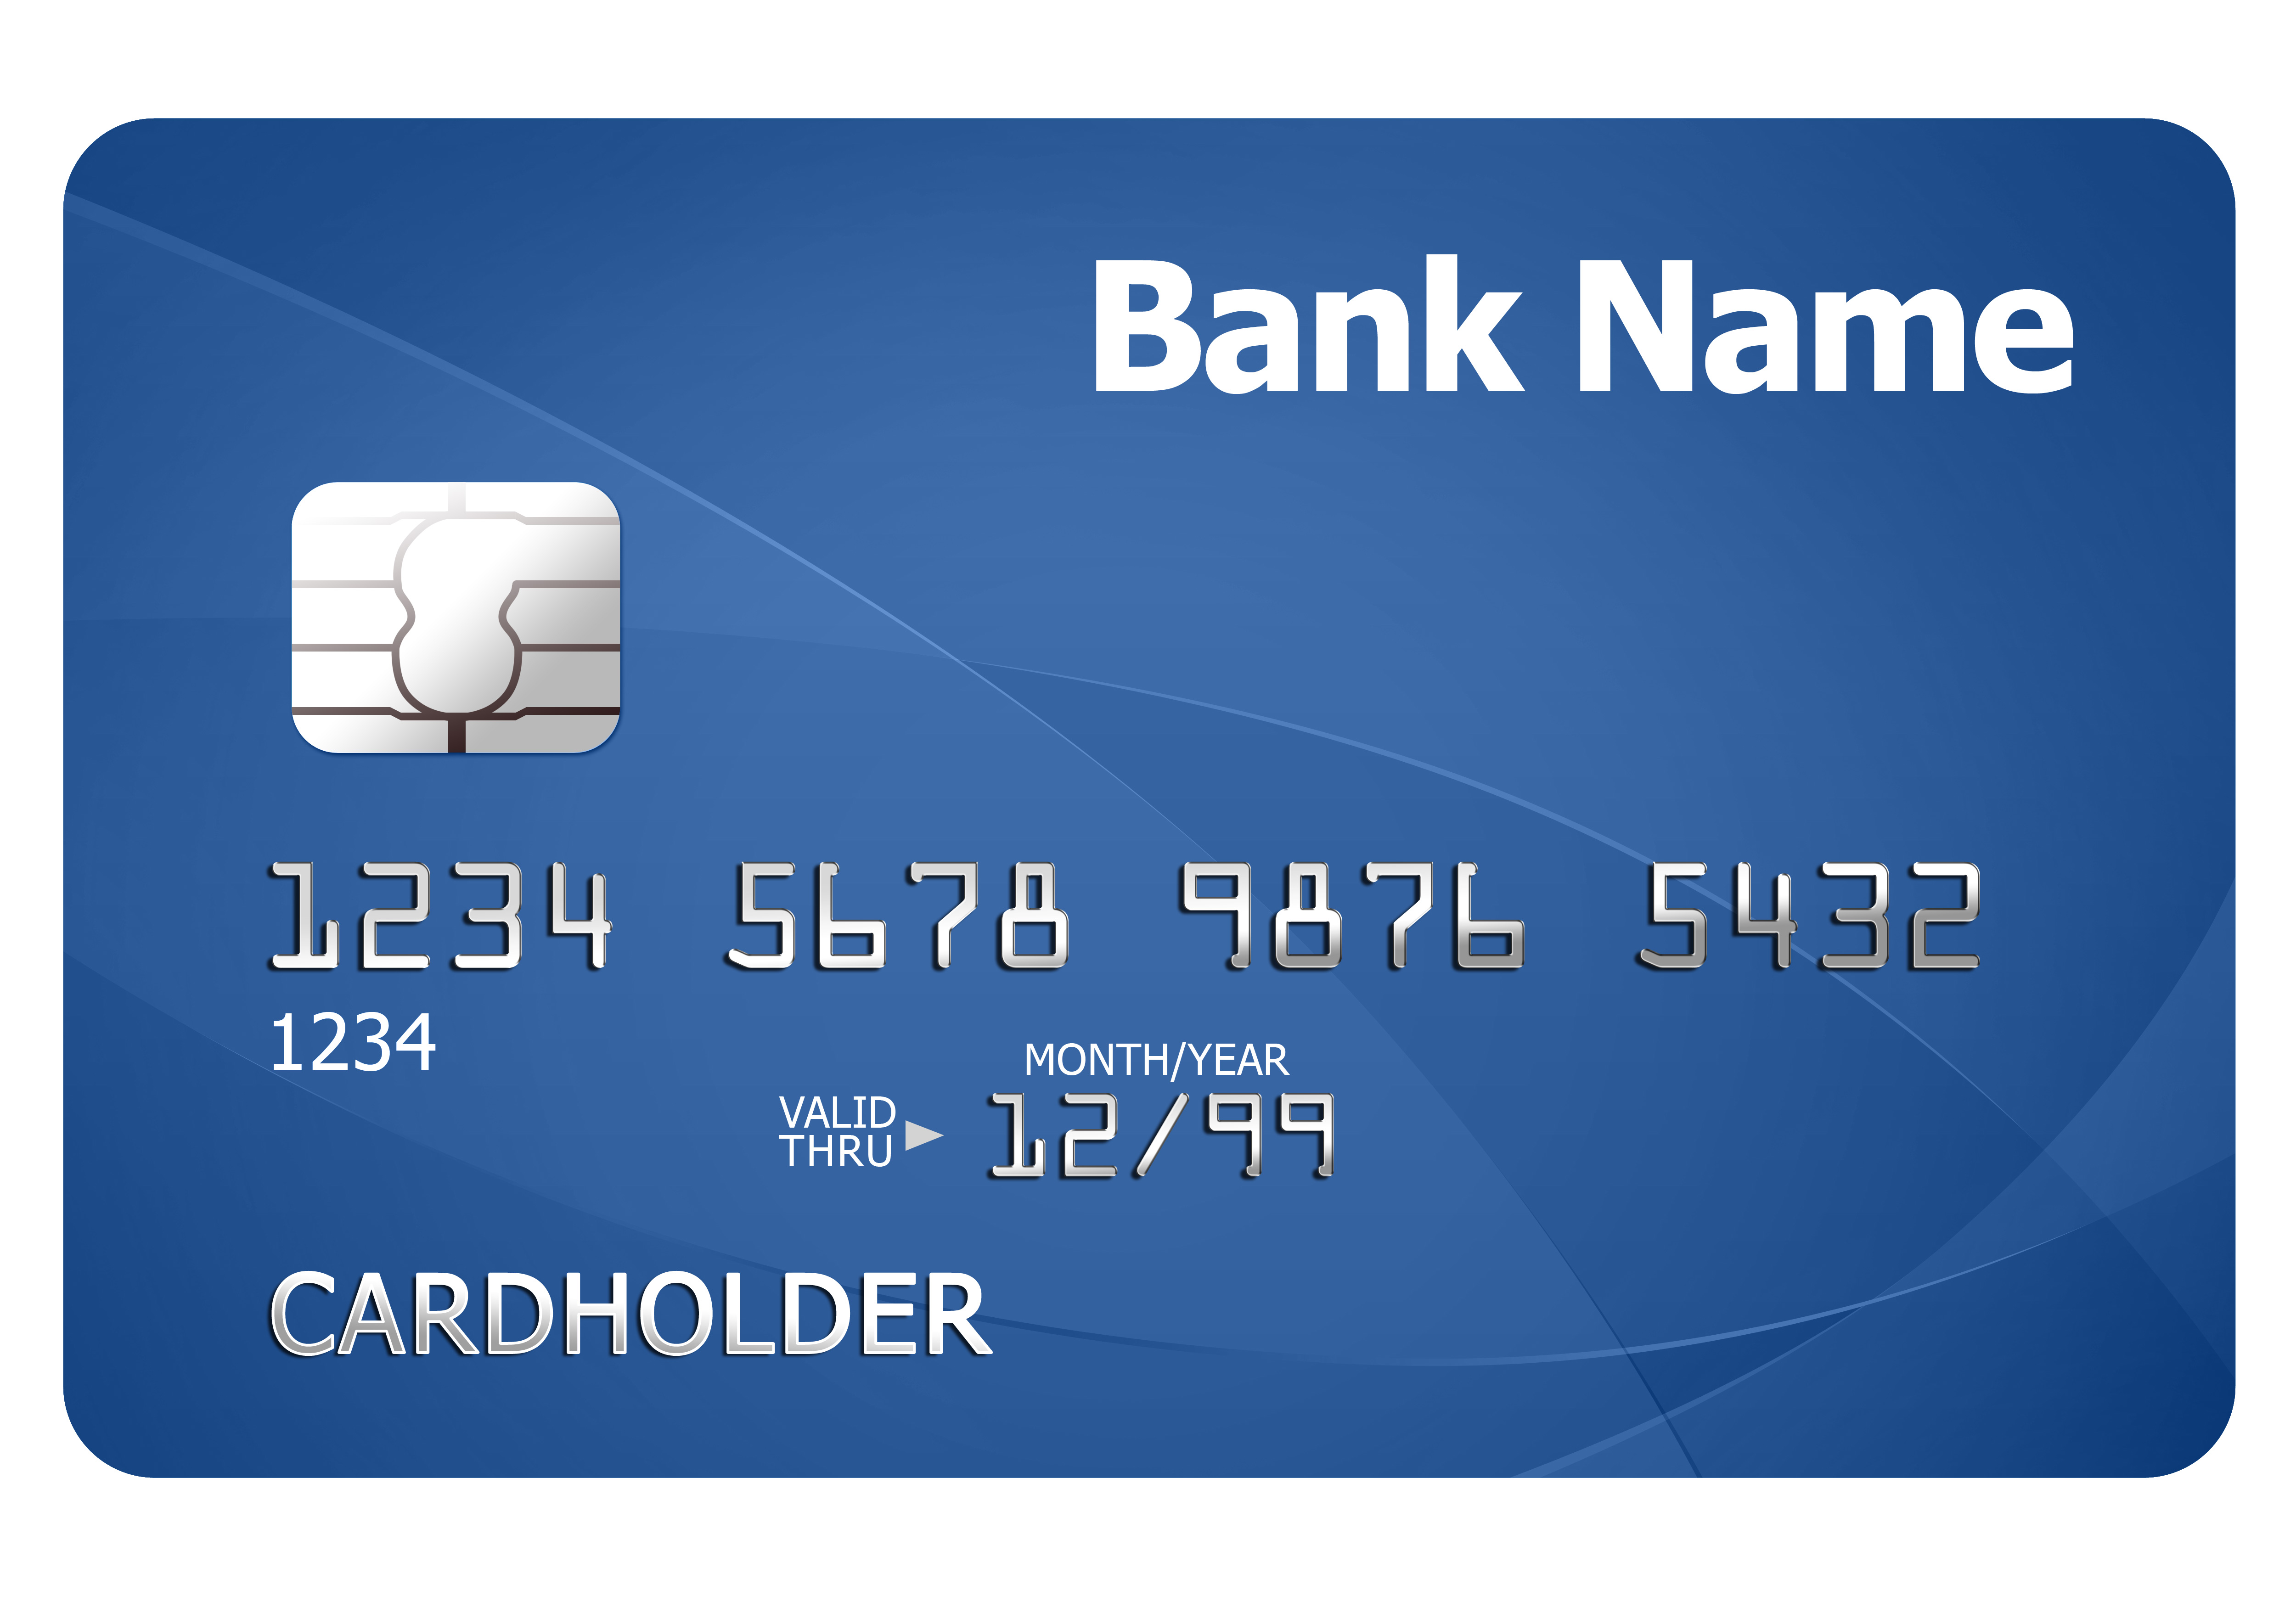
\includegraphics[scale=.03]{credit-card}
  \caption{Source: http://www.psdgraphics.com/psd/credit-card-template/}
\end{figure}
\end{frame}


\begin{frame}{Java Card - Architecture}
\begin{itemize}
\item Multilayered architecture
\end{itemize}
\begin{figure}[h]
  \centering
  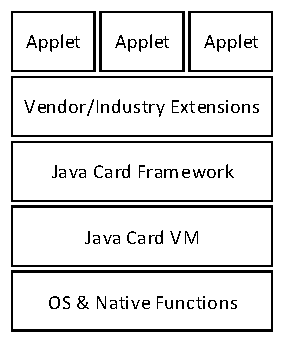
\includegraphics[scale=.7]{Architecture}
\end{figure}
\end{frame}

\begin{frame}{Java Card - Differences}
\begin{itemize}
\item A subset of Java:
  \begin{itemize}
  \item Only shorts, bytes, and booleans
  \item No threads
  \item No just-in-time compilation
  \end{itemize}
\item With additions:
  \begin{itemize}
  \item Firewall
  \item Transactions
  \end{itemize}
\end{itemize}
\end{frame}

% Skal måske ikke snakke om det her
% \begin{frame}{Java Card - Firewall}
% \begin{itemize}
% \item Multi-application smart card
% \item Separation is needed
% \end{itemize}
% \begin{figure}[h]
%   \centering
%   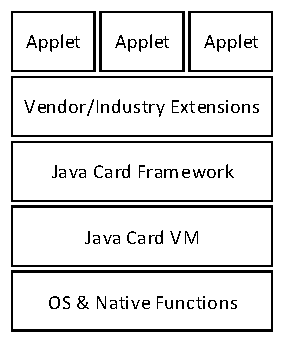
\includegraphics[scale=.7]{Architecture}
% \end{figure}
% \end{frame}

\begin{frame}[fragile]{TinyJCL}
  \begin{itemize}
  \item A number of bytecodes
  \item Based on Java Card language
  \item No type specific instructions
    \begin{itemize}
    \item Only values and addresses
    \end{itemize}
  \item Java Card applications can be rewritten in TinyJCL
  \end{itemize}
\end{frame}

\begin{frame}[fragile]{TinyJCL - New Instruction}
Old instruction
\scriptsize{
$$inst(P, mid, pc) = \texttt{IF\_CMPEQ }a$$
\[
    pc'= 
\begin{cases}
    a,& \text{if } x_{n-1} = x_n\\
    pc+2,              & \text{otherwise}
\end{cases}
\]
$$\inference[IF\_CMPEQ]{ops=(x_0, \ldots, x_{n-2}, x_{n-1}, x_n) \semsp ops'=(x_0, \ldots, x_{n-2})}
{CP, P \vdash \langle H, (CS, \langle mid, locals, ops, pc \rangle)\rangle \Rightarrow \langle H, (CS, \langle mid, locals, ops', pc' \rangle)\rangle}$$
}
\normalsize{New instruction}
\scriptsize{
$$inst(P, mid, pc) = \texttt{IF\_CMP}_{\phi} \text{ }a$$
\[
    pc'= 
\begin{cases}
    a,& \text{if } x_{n-1} \phi \text{ } x_n\\
    pc+2,              & \text{otherwise}
\end{cases}
\]
$$\phi \in \{ =, <, >, \leq, \geq, \neq \}$$
$$\inference[IF\_CMP]{ops=(x_0, \ldots, x_{n-2}, x_{n-1}, x_n) \semsp ops'=(x_0, \ldots, x_{n-2})}
{CP, P \vdash \langle H, (CS, \langle mid, locals, ops, pc \rangle)\rangle \Rightarrow \langle H, (CS, \langle mid, locals, ops', pc' \rangle)\rangle}$$}
\end{frame}

% Sprog/roed traad => Et eksempel i TinyJCL som skal gennemgaa i resten af fremlaegelsen
\begin{frame}[fragile]{TinyJCL Example}
\begin{lstlisting}[numbers=none, moredelim={[is][keywordstyle]{@@}{@@}}]
                            |  1. load 0               
1. boolean b = check();     |  3. invokevirtual #96     
                            |  5. store 6              
                            |  7. load 0
2. short sig = getSig();    |  9. invokevirtual #97
                            | 11. store 7
                            | 13. load 7
                            | 15. load 6
                            | 17. push 0               
2. if (b) {                 | 19. if_cmpeq 25               
3. Util.authorize(sig);     | 21. invokestatic #84
4. } else {                 | 23. goto 27
5.    Util.reject(sig);     | 25. invokestatic #85
                            | 27. return                  
}                           
\end{lstlisting}
\end{frame}
%%% Local Variables:
%%% mode: latex
%%% TeX-master: "AAUsimpletheme"
%%% End:
